\documentclass[11pt]{article}
\usepackage[a4paper,margin=1in]{geometry}
\usepackage{graphicx} %required to load images
\usepackage{mathtools} % required for sigma notation
\usepackage{amsmath} %required for the matrices
\usepackage{upgreek} %required for pi symbol
\usepackage{listings}
\usepackage{float}
\usepackage[utf8]{inputenc}
\usepackage{natbib}

\title{EE2703 Assignment 4: Fourier Approximations}
\author{Anvith Pabba EE19B070}
\date{5th March 2021}


\begin{document}

\maketitle

\section{Abstract}
In this assignment, We fit two functions \begin{textit}e^{x}\end{textit} and \begin{textit}cos(cos(x))\end{textit} over the interval [0,2*$\pi$) using the fourier series:

\begin{equation}
    a_0 + \sum_{n=1}^{+\infty} [a_n*cos(n*x) + b_n*sin(n*x)]
\end{equation}

\noindent In order to find the values of \begin{textit}a_n\end{textit} and \begin{textit}b_n\end{textit}, we use two different methods, These two methods are:
\begin{enumerate}
    \item Using the standard integration formulae
    \item Using \begin{textbf}lstsq\end{textbf} method to find the best fit coefficients
\end{enumerate}
We plot all the necessary graphs to visualise the data, and We then compare both sets of coefficients in the end.

\section{The Assignment}
\subsection{: Functions \begin{textit}e^{x}\end{textit} and \begin{textit}cos(cos(x))\end{textit}}

We first define functions that return its values as  \begin{textit}e^{x}\end{textit} and \begin{textit}cos(cos(x))\end{textit}, and we declare the input range (i.e the x values) from [-2*$\pi$ to 4*$\pi$).\\

But, a very important thing to note is that the function \begin{textit}e^{x}\end{textit} is \begin{textbf}{NOT}\end{textbf} periodic, while \begin{textit}cos(cos(x))\end{textit} \begin{textbf}{IS}\end{textbf} periodic.   And when we find the Fourier coefficients using the formulae, it assumes that the function is periodic. In this case, we take the period to be 2*$\pi$, and the periodic unit is from [0,2*$\pi$).\\

So, we now define two new functions that return its values as \begin{textit}e^{x}\end{textit} and \begin{textit}cos(cos(x))\end{textit}, but periodic with a period of 2*$\pi$. We can achieve this using a modulo function to cleverly give a periodic output. \\\\  Code is below:

\begin{verbatim}
#defining fuction for exponential
    def f(x):
    	return np.exp(x)
    
#defining function for cos(cos(x))
    def g(x):
    	return np.cos(np.cos(x))
  
#for periodic exponential and coscos  
    def f_periodic(x):
    	return f(x%(2*(np.pi)))
    
    def g_periodic(x):
    	return g(x%(2*(np.pi)))
\end{verbatim}

Below is the semilogy plot of periodic and non-periodic \begin{textit}e^{x}\end{textit}:

\begin{figure}[H]
    \centering
    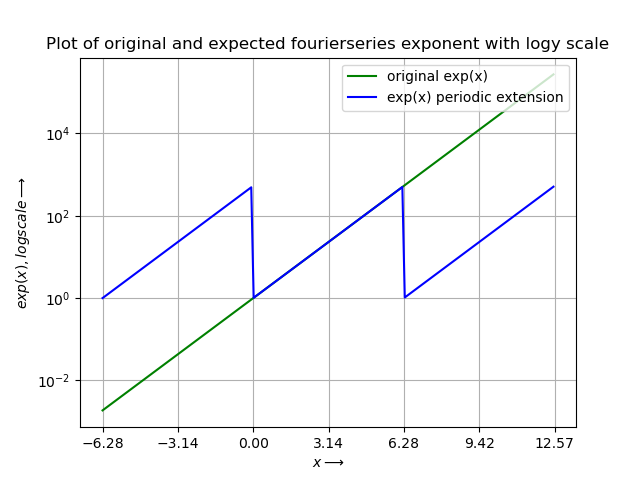
\includegraphics[scale = 0.5]{Figure_1.png}
    \caption{\begin{textit}e^{x}\end{textit} plots}
\end{figure}

\noindent and the plot of periodic and non-periodic \begin{textit}cos(cos(x))\end{textit}
Which are \begin{textbf}{BOTH THE EXACT SAME}\end{textbf}:

\begin{figure}[H]
    \centering
    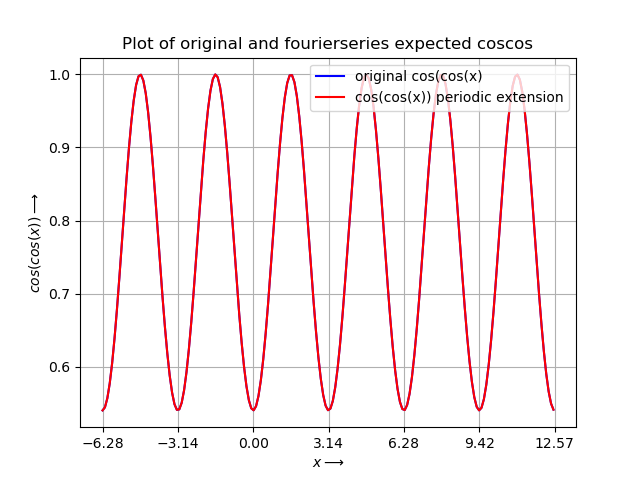
\includegraphics[scale = 0.5]{Figure_2.png}
    \caption{ \begin{textit}cos(cos(x))\end{textit} plots}
\end{figure}

\subsection{: Finding the Fourier coefficients using Integration}
The fourier series is :

\begin{equation}
    a_0 + \sum_{n=1}^{+\infty} [a_n*cos(n*x) + b_n*sin(n*x)] \approx f(x)
\end{equation}

the formulae to find these coeffients are given below

\begin{equation}
    a_0 = \frac{1}{2\pi} \int_0^{2\pi}f(x)\,\mathrm{d}x
\end{equation}

\begin{equation}
    a_n = \frac{1}{\pi} \int_0^{2\pi}f(x)cos(nx)\,\mathrm{d}x
\end{equation}

\begin{equation}
    b_n = \frac{1}{\pi} \int_0^{2\pi}f(x)sin(nx)\,\mathrm{d}x
\end{equation}

To integrate these in python, we use the builtin \textit{quad()} function to pass the extra \textit{k} argument to the function being integrated,
the syntax of \textit{quad()} is below:
\begin{verbatim}
    quad(u1,0,2*(np.pi),args=(k))[0]
\end{verbatim}

it outputs 2 values, with the first value being the value of the integration and the second being the error.\\
We now define functions with inputs x and k:
\begin{verbatim}
    #defining u1(x,k) and v1(x,k)
    def u1(x,k):
    	return f(x)*(np.cos(k*x)) #for a_n of exp(x)
    
    def v1(x,k):
    	return f(x)*(np.sin(k*x)) #for b_n of exp(x)
    
    #defining u2(x,k) and v2(x,k)
    def u2(x,k):
    	return g(x)*(np.cos(k*x)) #for a_n of coscos
    
    def v2(x,k):
    	return g(x)*(np.sin(k*x)) #for b_n of coscos

\end{verbatim}

\noindent python code to calculate the first 51 coefficients, and store all 51 of them in a vector C:

\begin{verbatim}
    A = np.empty([1,26], dtype = object)
    B = np.empty([1,26], dtype = object)

   #finding first 51 coeff of the above
    for k in range(1,26):
    	A[0][k] = (1/(np.pi))*quad(u1,0,2*(np.pi),args=(k))[0]
    	B[0][k] = (1/(np.pi))*quad(v1,0,2*(np.pi),args=(k))[0]
    
    A[0][0] = (1/(2*(np.pi)))*quad(f,0,2*(np.pi))[0]
    B[0][0] = (1/(2*(np.pi)))*quad(f,0,2*(np.pi))[0]
    
    C1 = np.empty([1,51], dtype = object)
    C1[0][0] = A[0][0]
    
    for i in range(1,26):
    	C1[0][2*i -1] = A[0][i]
    for j in range(1,26):
    	C1[0][2*j] = B[0][j]
    	
For coscos, change u1 to u2, v1 to v2, and C1 to C2.
\end{verbatim}
 \noindent We now plot the graphs of all the above Coefficients:
 \subsubsection{: Plots for Fourier coefficients of $e^{x}$}
 
 
\begin{figure}[H]
    \centering
    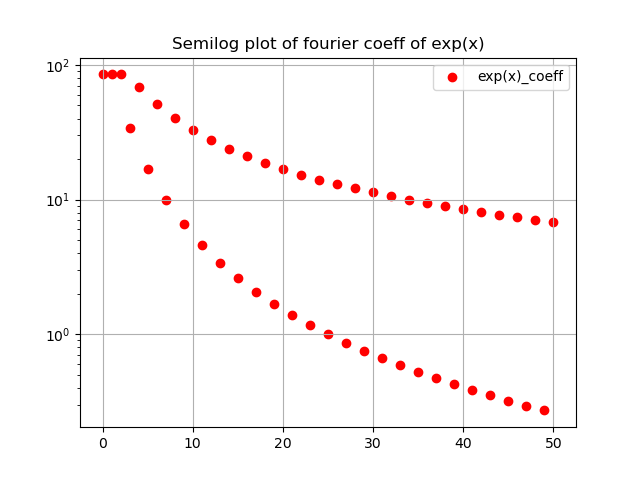
\includegraphics[scale = 0.5]{Figure_3.png}
    \caption{semilogy plot of $e^{x}$'s Fourier coefficients}
\end{figure}

\begin{figure}[H]
    \centering
    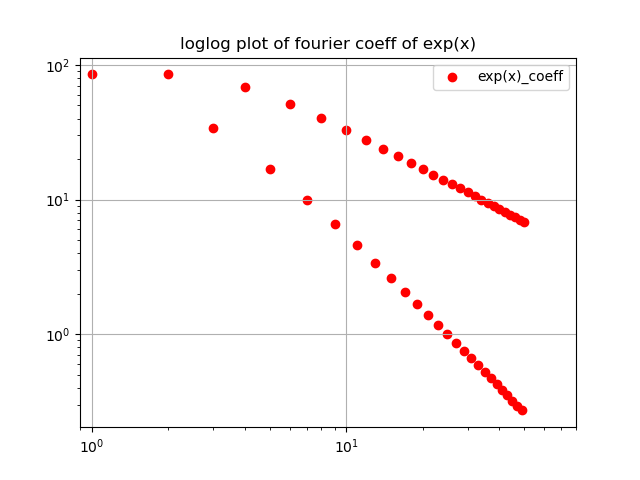
\includegraphics[scale = 0.5]{Figure_4.png}
    \caption{loglog plot of $e^{x}$'s Fourier coefficients}
\end{figure}

\subsubsection{: Plots for Fourier coefficients of cos(cos(x))}

\begin{figure}[H]
    \centering
    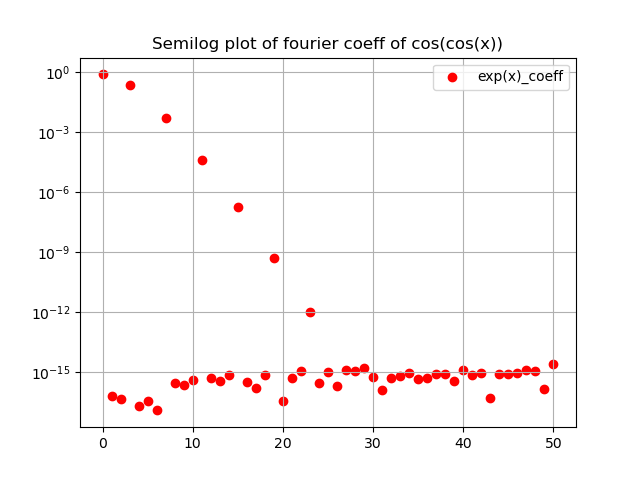
\includegraphics[scale = 0.5]{Figure_5.png}
    \caption{semilogy plot of cos(cos(x))'s Fourier coefficients}
\end{figure}

\begin{figure}[H]
    \centering
    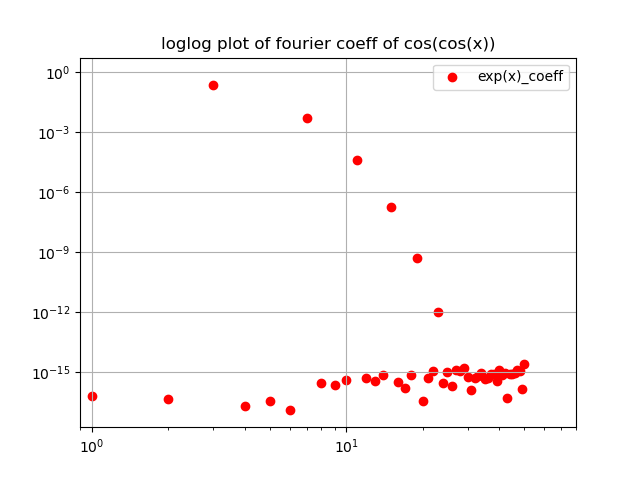
\includegraphics[scale = 0.5]{Figure_6.png}
    \caption{loglog plot of cos(cos(x))'s Fourier coefficients}
\end{figure}

\subsubsection{: Answering the questions in the Assignment}
a) If we look at Figure 5, we can see that many points are at the bottom near zero, this is because these points represent $b_n$  of cos(cos(x)) and as cos(cos(x)) is an \textbf{EVEN}, it is correct that $b_n$ is zero.\\

\noindent b)In the second case (i.e coscos), the function is naturally a periodic function that looks sinusoidal in nature, so it does not require as many harmonics, i.e the $a_n$ and $b_n$ die out quicker.\\
Whereas, for the first function, $e^{x}$ is \textbf{not periodic} and when we create the periodic extension, there exists a discontinuity. So, this discontinuity requires more harmonics, i.e the $a_n$ and $b_n$ do not die out quicker.\\

\noindent c)For $e^{x}$, the $a_n$ and $b_n$ decay proportional to $1/n^2$ and $1/n$. So the log of this coefficients is proportional to log(n), which is the scale of the axis, hence the loglog plot of the Fourier coefficients of $e^{x}$ is linear.\\
Whereas for coscos, the $a_n$ and $b_n$ decay exponentially with n, so the log of them is linear with respect to the x-axis. hence the semilogy plot of the Fourier coefficients of coscos is linear.

\subsection{: The least squares approach}
For this method, we us the lstsq method that we had learnt in the previous assignment. Here we have A.c = b, where the dimensions of A are 400x26, c is 26x1 and b is 400x1. To do this, we take 400 linear values of x from [0,$2\pi$) and find each and every respective value and fill up vectors A and b. We then use lstsq on the equation and find the vector c, which are the Fourier coefficients that best fit the function.

\subsubsection{: Code for the lstsq method}

\begin{verbatim}
    #Now for the "Least square approach"

    x=np.linspace(0,2*(np.pi),401)
    x=x[:-1] # drop last term to have a proper periodic integral
    b1=f(x) # f has been written to take a vector
    b2=g(x)
    A=np.zeros((400,51)) # allocate space for A
    A[:,0]=1 # col 1 is all ones
    for k in range(1,26):
    	A[:,2*k-1]=np.cos(k*x) # cos(kx) column
    	A[:,2*k]=np.sin(k*x) # sin(kx) column
    #endfor
    c1=np.linalg.lstsq(A,b1,rcond = None)[0] # the ’[0]’ is to pull out the
    c2=np.linalg.lstsq(A,b2,rcond = None)[0] # best fit vector. lstsq returns a list.
\end{verbatim}

\subsubsection{: Plot of lstsq calculated coefficients of $e^{x}$}

\begin{figure}[H]
    \centering
    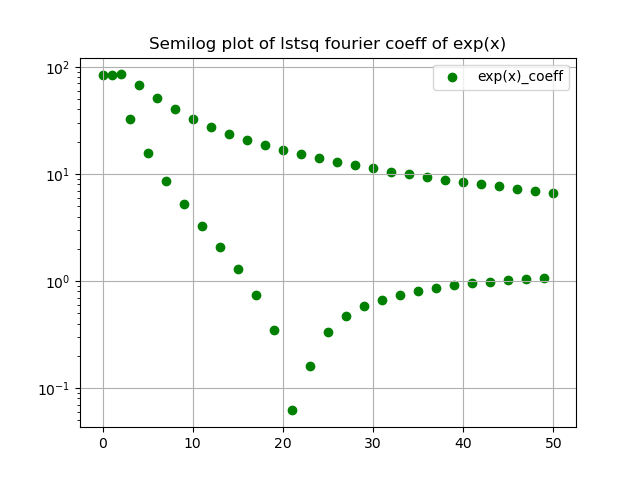
\includegraphics[scale = 0.5]{Figure_7.png}
    \caption{semilogy plot of lstsq $e^{x}$'s Fourier coefficients}
\end{figure}

\begin{figure}[H]
    \centering
    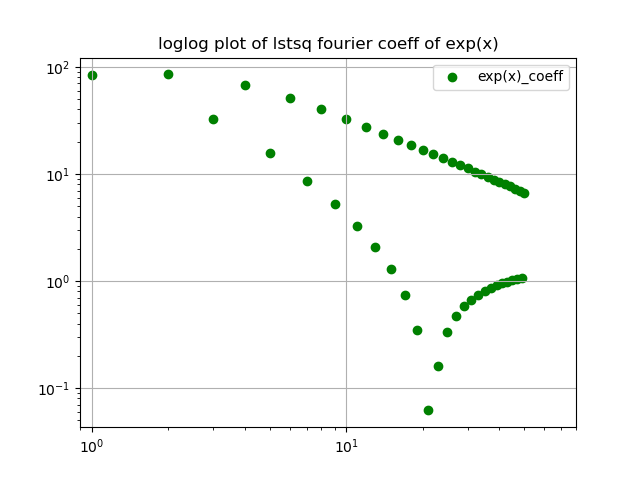
\includegraphics[scale = 0.5]{Figure_8.png}
    \caption{loglog plot of lstsq $e^{x}$'s Fourier coefficients}
\end{figure}

\subsubsection{: Plot of lstsq calculated coefficients of cos(cos(x))}

\begin{figure}[H]
    \centering
    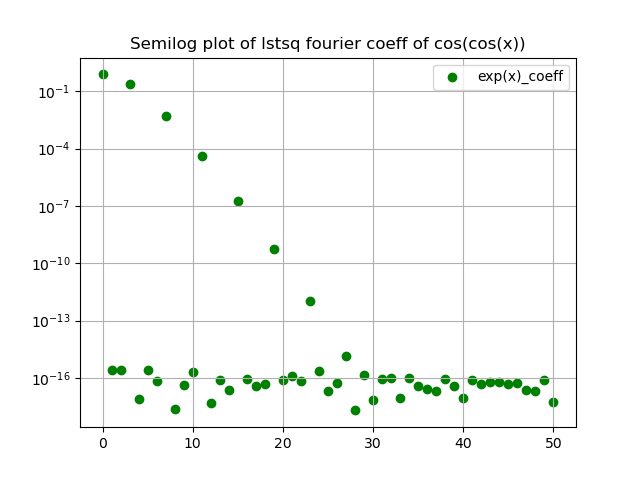
\includegraphics[scale = 0.5]{Figure_9.png}
    \caption{semilogy plot of lstsq cos(cos(x))'s Fourier coefficients}
\end{figure}

\begin{figure}[H]
    \centering
    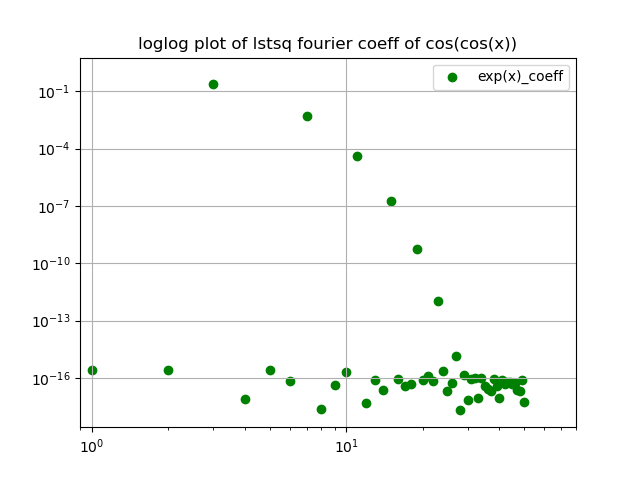
\includegraphics[scale = 0.5]{Figure_10.png}
    \caption{loglog plot of lstsq cos(cos(x))'s Fourier coefficients}
\end{figure}

\subsection{: Comparing the obtained Fourier coefficients}
\subsubsection{Absolute deviation}
A good way of visualising the deviation is by finding the absolute difference f both sets of coefficients and obtaining the maximum deviation.
\subsubsection{: Code for the above}
\begin{verbatim}
    #to find maximum absolute deviation

    c1_dev = np.absolute(c1 - C1)
    c2_dev = np.absolute(c2 - C2)
    
    def list_max(A):
    	max = 0
    	for i in range(len(A[0])):
    		if A[0][i] > max:
    			max = A[0][i]
    	return max
    
    c1_dev_max = list_max(c1_dev)
    print(c1_dev_max)
    c2_dev_max = list_max(c2_dev)
    print(c2_dev_max)

\end{verbatim}
\subsubsection{: Output}
After running the above code and printing the output, we get that the maximum absolute difference is : \\
\noindent For $e^{x}$ it is 1.3327308\\
\noindent For coscos it is 2.6 * 1e-15

\subsection{: Plotting the deviations of both sets of calculated coefficients}
To visualise the variations, let us plot both the sets in the same graph.

\subsubsection{: Plot of lstsq calculated coefficients of $e^{x}$}

\begin{figure}[H]
    \centering
    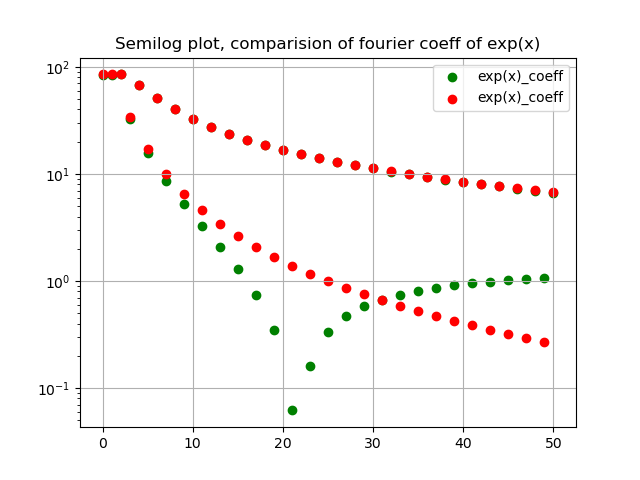
\includegraphics[scale = 0.5]{Figure_11.png}
    \caption{semilogy plot of both $e^{x}$'s Fourier coefficients}
\end{figure}

\begin{figure}[H]
    \centering
    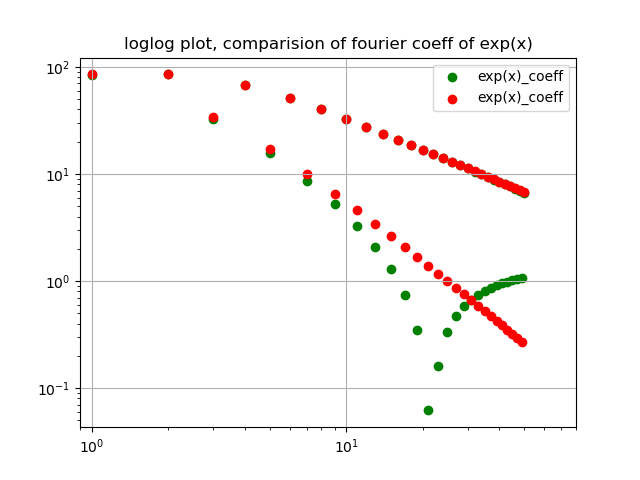
\includegraphics[scale = 0.5]{Figure_12.png}
    \caption{loglog plot of both $e^{x}$'s Fourier coefficients}
\end{figure}

\subsubsection{: Plot of both calculated coefficients of cos(cos(x))}

\begin{figure}[H]
    \centering
    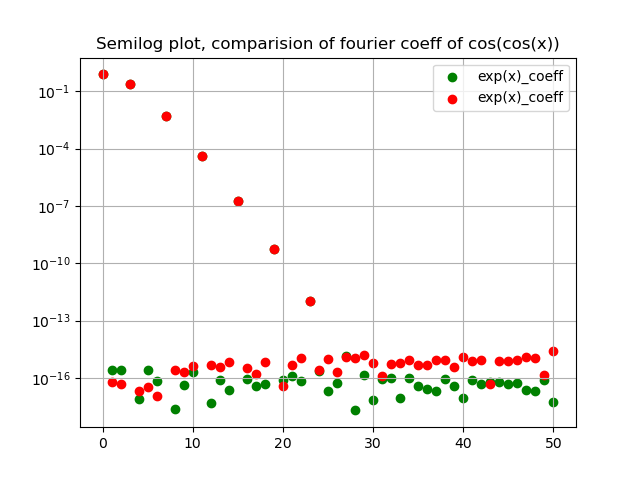
\includegraphics[scale = 0.5]{Figure_13.png}
    \caption{semilogy plot of both cos(cos(x))'s Fourier coefficients}
\end{figure}

\begin{figure}[H]
    \centering
    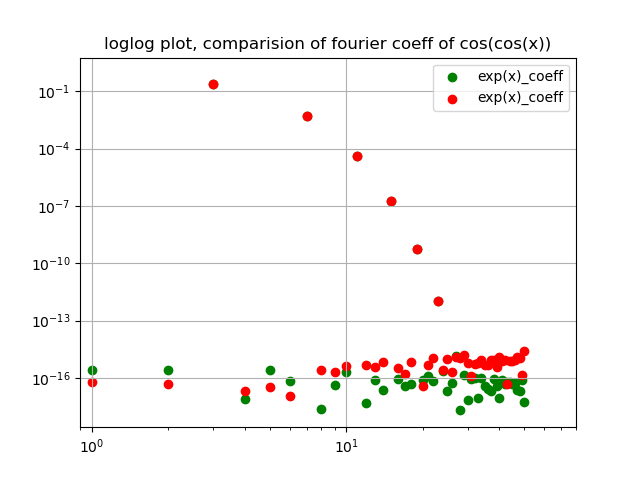
\includegraphics[scale = 0.5]{Figure_14.png}
    \caption{loglog plot of both cos(cos(x))'s Fourier coefficients}
\end{figure}

\subsubsection{: Answering the Assignment Questions}
When we look at all the above plots, we can see that the plots are very similar, but vary considerably in the Figure 11 and 12 (i.e the plots of $e^{x}$). The reason for this is that the lstsq method fits the best values of the first 51 Fourier coefficients while also trying to compensate for the missing harmonics.\\
\\As $e^{x}$ has a discontinuity, it requires more number of harmonics to be accurate.\\
\\In the case of finding the coefficients via integration, the coefficients are found without compensating for the lack of harmonics.\\
\\As coscos doesn't require many harmonics, both the calculated coefficients are almost the same, whereas for $e^{x}$, there is a variation.\\
\\Hence if we increase the number of calculated coefficients from 51 to something very high like of the order $10^7$, then the deviation of both the graphs would decrease substantially.

\subsection{Calculating and plotting A.c}

\subsubsection{: Code To calculate output of A.c}
\begin{verbatim}
    Ac1 = np.dot(A,c1)
    Ac2 = np.dot(A,c2)
\end{verbatim}

\subsubsection{: Plotting the A.c values with the actual functions}

plot of A.c1, $e^{x}$ periodic and non-periodic:
\begin{figure}[H]
    \centering
    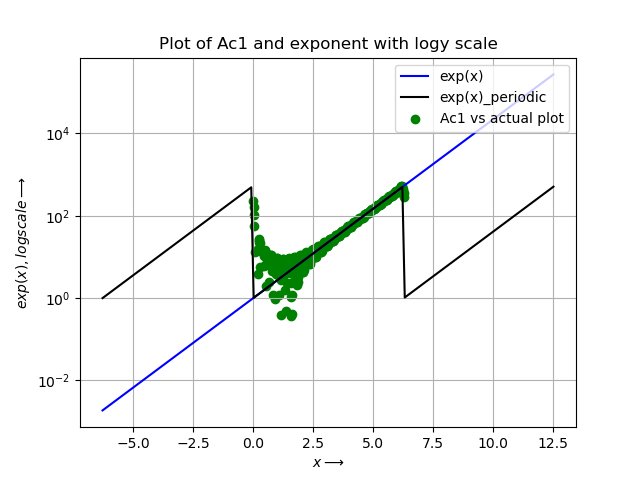
\includegraphics[scale = 0.5]{Figure_15.png}
    \caption{plot of calculated and actual $e^{x}$}
\end{figure}

plot of A.c2, actual coscos:
\begin{figure}[H]
    \centering
    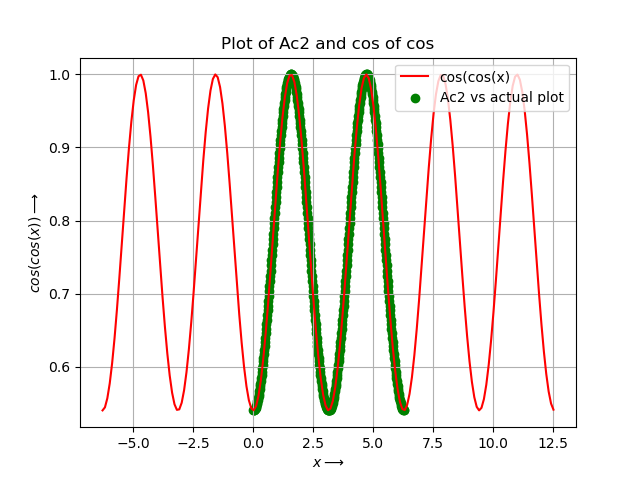
\includegraphics[scale = 0.5]{Figure_16.png}
    \caption{plot of calculated and actual coscos}
\end{figure}

\subsubsection{: Answering the Assignment Questions}
We can see that the expected and calculated values of coscos are the same, but the expected and calculated values of $e^{x}$ vary near the point of discontinuity. This phenomenon is known as Gibbs phenomenon, and it is defined as "The overshoot (or "ringing") of Fourier series occurring at simple discontinuities." And this overshoot at the discontinuity doesn't die out for very high finite n.

\section{Conclusions}
In this Assignment, I've learnt :
\begin{itemize}
    \item How to integrate a function in python
    \item How to use lstsq method to find the coefficients that best fit
    \item How to calculate the Fourier coefficients through different methods
    \item About Gibbs phenomenon and a how Fourier series reacts to a discontinuity.
\end{itemize}


















\end{document}
